\documentclass[declaration,shortabstract,english,inz]{iithesis}
\usepackage[utf8]{inputenc}

%%%%% Tittle page
\polishtitle    {Tworzenie agenta kierującego pojazdem w wirtualnym środowisku TORCS}
\englishtitle   {Developing car driving agent in the TORCS virtual environment }
\polishabstract {\ldots}
\englishabstract{\ldots}
\author         {Kacper Kulczak}
\advisor        {dr Paweł Rychlikowski}
% \date          {}                      %Date
\transcriptnum {279079}
\advisorgen    {dr. Pawła Rychlikowskiego}
%%%%%

%%%%% packages
\usepackage{
    graphicx,
    listings,
    hyperref,
    array,
    longtable,
    wrapfig,
    amsmath,
    algorithmic
    % amssymb,
    % amsthm,
    % amsfonts,
    % tikz 
}
%%%%% Definitions and commands
%
%\theoremstyle{definition} \newtheorem{definition}{Definition}[chapter]
%\theoremstyle{remark} \newtheorem{remark}[definition]{Observation}
%\theoremstyle{plain} \newtheorem{theorem}[definition]{Theorem}
%\theoremstyle{plain} \newtheorem{lemma}[definition]{Lemma}
%\renewcommand \qedsymbol {\ensuremath{\square}}
% ...
%%%%%

\begin{document}

%%%%% BEGINNING

\chapter{Introduction}

Autonomous cars are very trendy subject nowadays. The idea has a lot of benefits. Most of accidents on roads, occurs due to human mistakes. Programmes don't get tiered or distracted while driving a vehicle. Also they can save a lot of fuel with optimal decisions.
That's why companies around the globe put a lot of effort into making the car software for autonomous driving. It is very interesting task from artificial intelligence perspective. Description of the world is huge. It includes near objects, borders of the street, speed, turning force, engine rotation and much more. The output of such programme is quite simple in compared to the input size. We need only to specify new position of steering wheel and decision if we want to speed up or slow down. During my work I wanted approach the problem by building my own agent capable of drive safely on a racing track.




\section{TORCS Environment}
"The online racing car simulator"(TORCS) is very accurate car simulator with 3D graphic engine. It allows to run races with various cars and tracks. The simulation features a damage model, fuel consumption, aerodynamics, wheel properties, aerodynamics, advanced slipping model and much more \cite{TORCS}.  It is designed to enable programed agents compete against each others. There is very detailed instruction on developing your  own bot. It has to be written as C++ loadable library and it is attached to main thread during program startup.


\begin{figure}[h]
    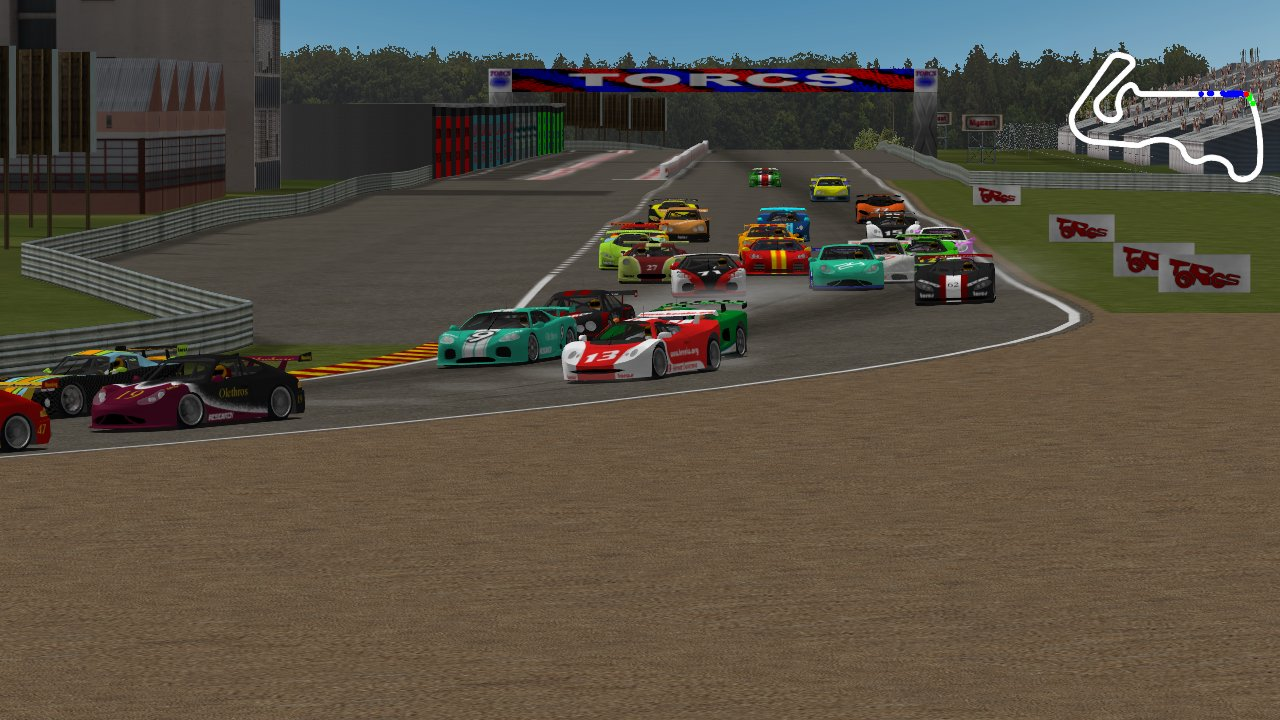
\includegraphics[width=\linewidth]{img/torcs_look.jpeg}
    \caption{Screen shot from TORCS race \cite{TORCS}}
    \label{fig:torcs}
\end{figure}
I have much more experience with programming in high level languages, so clean TORCS environment did not meet all my expectations. 


\section{Simulated Car Racing Championship}

SCRC competition took place between 2007 - 2015 with some breaks. It was organized by the University of Adelaide and the Politecnico de Milano. They used TORCS engine for competition, but organizers provided official patch which changed architecture of the programme. After patching, TORCS became client-server application which allows multiple bots communicate with game engine via UDP connections. 

\begin{wrapfigure}{R}{0.6\textwidth}
    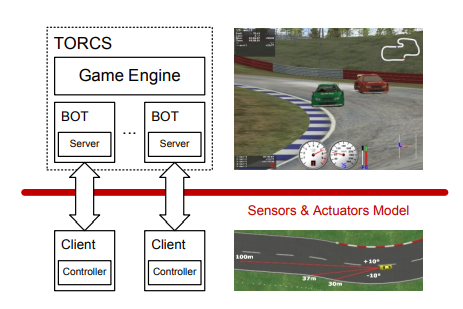
\includegraphics[width=0.55\textwidth]{img/scr_architecture.png}
    \caption{Simulated Car Racing Championship - architecture overview \cite{scrc_manual}}
    \label{fig:scrc_arc}
\end{wrapfigure}

Server sends current sensor inputs (track border, speed, lap time, etc...) and waits for 10ms for the client action (gas, break, steer, etc...). API is details are descrived in table from manual. With that change participants cant choose whatever language they want. That's why I decided to use patched version of TORCS game engine in version 1.3.7

Organizers provided "clients" programmes only in Java and C++. I didn't want to implement communication interface on my own, beacuse it's time consuming  and uninteresting task. After some research,  I found \url{http://xed.ch/p/snakeoil} project, which provides Python Class handling communication with TORCS server. It allowed me to add layer of abstraction and focus directly on driving functionality.

\section{Game sensors and actions parametes}
    
Server provides very accurate description of virtual environment state. All sensors used by ma agents are described in tables \ref{tab:torcs_sensors} \ref{tab:torcs_actions}.
Full list of parameters provided by game engine can be found in SCRC competition manual \cite{scrc_manual}. Sensors allow to determined exact car position on the track, and also predict close future shape of the track.


\begin{center}
    \begin{longtable}{ | p{0.18\textwidth} |p{0.25\textwidth}| p{0.45\textwidth} |}
     \hline
     \textbf{Name} & \textbf{Range (unit)} & \textbf{Description} \\ 
     \hline
     angle & $[-\pi, +\pi]$ (rad) & Angle between the car direction and the direction the track axis. \\  
     \hline
     distFromStart & $[0, +\infty)$ (m) & Distance of the car from the start line along the track line. \\
     \hline
     gear & $ \{ -1,0,1, \dots, 6 \} $ & Current gear: -1 is reverse, 0 is neutral and the gear from 1 to 6. \\
     \hline
     speedX & $ ( -\infty, +\infty ) $ (km/h) & Speed of the car along the longitudinal axis of the car. \\
     \hline
     speedY & $ ( -\infty, +\infty ) $ (km/h) & Speed of the car along the transverse axis of the car. \\
     \hline
     speedZ & $ ( -\infty, +\infty ) $ (km/h) & Speed of the car along the Z axis of the car \\
     \hline        
     track &  $[0, 200]$ (m) & Vector of 19 range finder sensors: each sensors returns the distance between the track edge and the car within a range of 200 meters. \\
     \hline
     trackPos & $( -\infty, +\infty )$ & Normalized distance between the car and the track axis. Values beetwen $[-1, 1]$ means that the car is on the track. \\
     \hline
     wheelSpinVel & $[0, +\infty)$ (rad/s) & Vector of 4 sensors representing the rotation speed of wheels. \\
     \hline
     \caption{\label{tab:torcs_sensors}: Description of the available sensors. Cited from \cite{scrc_manual}}
    \end{longtable}

\end{center}

\begin{center}
    \begin{longtable}{ | p{0.18\textwidth} |p{0.22\textwidth}| p{0.5\textwidth} |}
    \hline
    \textbf{Name} & \textbf{Range (unit)} & \textbf{Description}  \\ 
    \hline
    accel & $\{0,1\}$ & Gas pedal \\ 
     \hline
     brake &  $\{0,1\}$ & Brake pedal \\ 
     \hline
     gear & $\{-1,0,1,\dots ,6\}$ & Gear value \\ 
     \hline
     steer &  $[-1,1]$ & Steering value: $-1$ and $+1$ means respectively full right and
     left \\ 
     \hline
     \caption{\label{tab:torcs_actions}Description of the available  action parameters. Cited from \cite{scrc_manual}}
    \end{longtable}
\end{center}

\chapter{Heuristic approach}

\section{Line follower}

The first approach to the problem was developing simple bot which follows the track axis. Every time, absolute value of trackPos sensor (normalized position of the car on the track between $[-1, +1]$) is bigger than given small threshold, agent turns towards axis of the track with turning force set to 35\%. To avoid zigzag driving, very small course corrections are applied, whenever $abs(trackPos) < 0.2$. Speed is limited to 80 km/h. Several configurations of constant parameters were tested and current configuration allows bot to safely drive on every track. 

I am aware that limiting turing force, has huge negative impact on bot performance. However increasing that value leads to dangerous behaviors. I was surprised how easy it is to slip. During development line follower I haven't found any solution for getting out of the slip. For now limiting that value was necessary.

\section{Speed limit signs}

In real world, government for safety reasons, places speed limit sign on dangerous sectors of roads. Signs are placed before sharp turns, steep slopes, bridges, viaducts, and more. Drivers adjust the speed to specific environment conditions. Inspired by this observation, I tried to improve previous agent iteration. 

I've split the track on 8 sections, using distFromStart sensor (distance of the car from the start line along the track line). Every part would have different speed limit set for specific track. The goal is to finish the lap as fast as we can while not falling out of the track. So we need to minimize function $f$, where $l_i$ - speed limit for section $i$ in km/h.

$$ f(l_1, l_2, \dots, l_n ) =  \begin{cases}
    \infty, &\quad \text{when the car fell off the track}\\
    \text{lap\_time}, &\quad \text{otherwise} \\
  \end{cases}
 $$

I was trying to implement genetic algorithm for finding optimal limits for given track, but it appears that game engine, even with turned graphics off, isn't as fast as I anticipated. It takes almost 20 seconds, to complete one lap. Simple genetic algorithm would need long hours to find approximately good solution. I've used two following observations while developing my algorithm.

\begin{itemize}
    \item  $l_i \in [40, 300]$:  Smaller values can lead to disqualification from race.
    \item  true speed of car on section $i$, depends on $l_i$ and true speed at the end of section $i-1$
    \item
    $l_i$ is correct, when $l_{i+1} = 40$ and car didn't fell out from track
    \item  $g_j(x) = f(l_1,l_2, \dots,l_{j-1}, x, l_{j+1}, \dots, l_n)$ is decreasing while car stays on the track
    
\end{itemize}


I've implemented algorithm based on divide and conquer idea. It finds maximal x, where $g(x) \neq \infty$. We run that procedure on every argument:

\begin{algorithmic}
    \STATE $l_i\gets 40$
    \FOR{$i\gets 1,\dots, n$}
        \STATE $l_i = devide\_and\_conquer(func=g_i, min=40, max=300)$
    \ENDFOR
\end{algorithmic}

For every section it uses around 12 game engine runs. So whole algorithm ends execution after around half an hour.

\section{Results and observations}

In following table I've presented line-follower performance on specific tracks from TORCS environment. While speed limits are significant improvement, they still do not deal with major flaw of the concept. Our bot is extremely reactive. Human driver see a turn from distance and prepares for it (reduces speed, drifts towards opposite side of the road). On the other hand my bot turns the steering wheel only when it drifts away from the middle of the track (this happens after entering the turn). It is basically to late for a perfect turning maneuver. We need a model, which predicts and reacts to the  future events. That's why I resign from extending current concept.


\begin{table}[h]
    \centering
    \begin{tabular}{ |c|c|c|c|}
          \hline
          track name & unexperienced human[s] & line-follower[s] & speed limits[s]  \\
          \hline
          forza &  $122.65$ & $265.51$ & $146.31$   \\
          \hline
          cg\_track\_2 & $79.64$ & $148.84$ &  $84.68$  \\ 
          \hline
          cg\_track\_3 & $102.09$ & $133.74$ & $91.86$   \\
          \hline
        \end{tabular}
        \caption{Line follower performance for specific TORCS tracks}
        \label{tab:line_follower}

\end{table}

\chapter{Machine Learning Approach}

\section{Introduction}


For very complex tasks creating an algorithm can be very challenging.
 Most of the time we have an input, we define requirements and develop an algorithm which solves our problem. But sometimes the task is to complex to be solved by an algorithm designed by human. In that case programmes can use machine learning. For example let's take email spam detection. Users get a lot off unwanted messages on their emails, most of the time they delete just them and that's a great thing. They unconsciously provide a labeled data sets, on which we can test our solution. Creating algorithm which predicts if a message is spam is extremely difficult. We can check for existence of specific keywords, measure length, check upper case letters appearance, but combining all this variables needs a lot of testing.

 Instead of that, we can try to extract statistical relations in collected data. Machine learning algorithms can be applied when we have algorithm input and expected output for every example in the data, but we have no idea how it should be achieved. We receive not optimal, but approximately good solution for our problem and that's exactly what we want from spam detector. It should help users in omitting unwanted messages, but it's not a problem if he is wrong.

 Primary machine learning problem is classification\cite{Introduction_ML}. We want to assign every input to one of given classes. In our email example we've got two classes (SPAM, NOT-SPAM), but we can have much more of it. Model designed to solve that type of problems is called classifier. Quality of classifier can be measured by percentage of correctly predicted classes on the test data sets.

 Problems where output is a single floating point number are called regression \cite{Introduction_ML}. Model which predicts price of car is much more useful thant one which assigns car to one of following classes  (cheap, medium, expensive). Such models are called regressors and we can measure their quality by counting mean squared error between real and predicted values on the test data set.

In some problems, single action don't have huge impact on result. An action is good only as a part of good policy. Methods which focus on that approach are called reinforcement learning \cite{Introduction_ML}. Car driving can be classified as such problem. Sometimes there isn't optimal action for current situation, it is rather optimal sequence of action which gives positive result.


\section{Applying machine learning for car driving problem}

Accuracy of machine learning models depends heavily on amount of collected data. Trains data set should describe whole space of problem variables. With plenty of data samples we can extract most meaningful dependencies and predict outputs on real life data samples. However recent work by P. Dybiec \cite[2018]{rover}, which focuses on autonomous driving developed for martian rover shows that, it is possible to successfully apply machine learning technics with relatively small data set. 
  
I don't have access to huge database of car driving logs, but during agents development I became well TORCS driver. So I decided to record my performance on race tracks.

Unfortunately TORCS environment does not have an option to log sensors data and driver actions. It is planned to add this functionality in the future development. That's why I developed software which mimics TORCS car controls and saves data from all sensors and driver actions to json file. From game perspective it is normal agent, but it reacts only on user keyboard inputs (accelerate, break, left, right).  With that infrastructure During 25 recording laps on \textit{cg\_track\_2}, I've collected around 55000 data frames (description of car state and driver action, saved every 10ms).

\section{Single model agent}



First machine learning approach was to develop simple model which predicts action for every data frame during the race. Input consist of all state sensors described  in \ref{tab:torcs_sensors} and normalized to fit in range $[-1,1]$. To determine classes of actions, I've extracted all unique actions taken by the driver and then labeled them, to generate simple classification problem.
\paragraph{Action parameters}
\begin{itemize}
    \item \textbf{accel} $\in \{0,1\}$
    \item \textbf{brake} $\in \{0,1\}$ 
    \item \textbf{steer} $\in [-1,1]$
\end{itemize}
After splitting the data on train and test data set, I've trained classifiers to predict the best action for current car situation. I've used algorithms implemented scikit-learn \cite{scikit_learn} library. Results of experiments are shown in table \ref{tab:single_clp_tree}


I've started with simple Decision Tree classifier. CART (classification and regression tree) algorithm produces binary tree which consist of decision nodes and terminal leafs. Every node holds a binary condition (for example $\textit{angle} > 0.37$) which passes data frame to one of it's children. Every leaf is labeled by class which it represents. To classify specific input we traverse a path directed by decision nodes. To choose variable and value used in condition creation we are minimizing impurity function. More detailed description can be found in \cite{Introduction_ML}.

Second model used was Random Forest. It contains multiple decisions tree, constructed with randomized algorithm (in my experiment, 40 trees). To predict class of data point, we average predictions from all trees in the model \cite{Introduction_ML}. 

\begin{table}[h]
    \centering
    \begin{tabular}{ |c|c|c|c|}
          \hline
          agent & cg\_track\_2 result [s] & train score & test score \\
          \hline
          speed\_limits & $84.68$ & - & -\\
          \hline
          CART &  $63.25$ & $0.81$ & $0.65$\\
          \hline
          Random Forest & $65.39$ & $0.99$ & $0.66$ \\
          \hline
          
        \end{tabular}
        \caption{Single Model:agents performance}
        \label{tab:single_clp_tree}

\end{table}


Despite poor accuracy on test models, performance was improved by almost 25\%, compared to heuristic agent with speed limits. Difference between train and test score is large, so models are overfitted. Anyway, agent can recreate enough human actions, to stay on well known part of track. 

It is worth noticing, that using \textbf{distFromStart} (distance from start line according to track middle line) parameter isn't very practical for generalized driving agent. My models weren't learning how to drive a vehicle. The were rather memorizing right actions for specific sector of the track. We need model which can be applied also for unseen tracks. However without that parameter, all my models were crashing on the track. They were able only to apply similar actions in similar places.

\section{Two models agent}

Major flaw for previous one model agent was tha amount of classes used in classification. Data set is too small for such variety of decisions. To simplify classification task I've decided to use two separate models: 

\begin{itemize}
    \item \textbf{Steer Regressor} - responsible for determining the turn rate (floating number between [-1,1]).
    \item \textbf{Acceleration Classifier} - responsible for choosing one of three speed actions \{accelerate, do\_nothing, brake\}
\end{itemize}

State vector for regressor is the same as on used in single model approach. Classifier input is expanded by \textbf{steer} value predicted by the regressor. Intuition behind passing value between two models is that, breaking and accelerating during turning the manoeuver, leads to dangerous behaviors. Humans tends to reduce the car speed before beginning of the turn. Acceleration classifier should depend on expected steering decision.


This time I've used MLP (Multi Layer Perceptron) implemented in scikit-lirary \cite{scikit_learn}. It is simple neural network model which need more time to train, but is much more powerful than simple decision trees. 
!!! DWSCRIBE NEURAL NETS!!!

Because of hardware limits I was able to train very simple networks regressor hidden layers (300,30); classifier hidden layers (200,20) both with hyperbolic tangent activation function). Input data have all parameters from single model agent, instead of \textbf{distFromStart} parameter. All of them are standardized in range [-1,1].

\subsection{Architecture motivations}

There were two observations in advantage of this architecture. 

First of all, it significantly reduces amount of classes used in classifier. Three classes should be covered effectively with amount of collected data.

Secondly with steer parameter determined by classifier we encounter following problem with penalty for learning algorithm. Let's say we've got data sample with, action taken by human driver, to $steer=0.5$. Consider two wrongly predicted answers by models:
\begin{itemize}
    \item[a)] $steer=-0.4$
    \item[b)] $steer=0.35$
\end{itemize}

For classification problem both predictions (a and b) are equally wrong.  The class prediction is just missed. However for reconstructing steering actions case b) is much worse and more dangerous than a). When we are near edge of the track, that kind of wrong prediction can lead as away from the track resulting in a crash. When we approach setting \textit{steer} as regression problem we tends to choose values which are close to real ones. Regressor more accurately reflects steering actions which appears in the data set.

\subsection{Results}

\begin{table}[h]
    \centering
    \begin{tabular}{ |c|c|c|c|}
          \hline
          agent & cg\_track\_2 result [s] & train set & test set \\
          \hline
          \textbf{double agent} & DNF &   &  \\
          \hline
          Steer regressor error [MSE]&   & $0.0041$ & $0.0043$\\
          \hline
          Acceleration classifier score [\%]&  & $0.99$ & $0.98$ \\
          \hline
          \textbf{double agent - joined state} & DNF &   &  \\
          \hline
          Steer regressor error [MSE]&   & $0.0026$ & $0.0028$\\
          \hline
          Acceleration classifier score [\%]&  & $0.99$ & $0.98$ \\
          \hline
          
        \end{tabular}
        \caption{Double models agents performance}
        \label{tab:double_models_results}

\end{table}


Models were trained on from single agent approach (without \textbf{distFromStart} sensor). Accuracy of models on testing set is quite reliable \ref{tab:double_models_results}. That's the effect of reducing number of actions classes. However agent is unable to finish the lap on training track. It appears that steering regressor isn't effective enough. 

!!!! Paagraph about prev state !!!!

One of ideas to improve these agent, was assumption that, maybe planning driving policy is impossible with only one data frame processed at once. To take into account longer period of time, agent remembers state and action from previous time frame and attaches it to both models inputs. Results of the experiment are shown in second part of table \ref{tab:double_models_results}. New approach allows to reduce mean squared error twice of steering regressor on data sets. However, agent driving is very aggressive. It includes a lot of sharp steering wheel turns even on straight sections of track. It is still unable to reach the finish line without a crash.

Even with significant improvement in accuracy, models are still not capable to drive safely on the track. Racing cars, drives extremely fast and one sharp turn in opposite direction, can causes inevitable crash situation. There is no place for such mistakes.  

\section{Three model agent}

I've been observing previous models performance and I've came to conclusion that biggest problem occurs when agent unexpectedly steer sharply in opposite directions. Steering regressor accuracy is measured on absolute distance between magnitude of output and real steering value. It does not take into account steering direction, so we need to put more effort in correctness of that decision.

\subsection{Steering supervision}


\textbf{Steering supervisor} classifier is supposed to reduce amount of missed steering directions decisions. Input for this one is the same as other models. Training output is extracted from data set by applying function $f$ on \textbf{steer} value from driver actions. 
$$ f(steer) =  \begin{cases}
    sign(steer), &\quad steer\neq0 \\
    0, &\quad \text{otherwise} \\
  \end{cases}
 $$


To predict \textbf{steer} value we compute $m$ which is output of steering regressor and $d$ which is output of steering supervisor. Then we apply function $g$ for those values, and that's our final \textbf{steer} value. Function $g$ passes $m$ only when both models agreed on turning direction. Also when supervisor predicts no turning action, $g$ decreases $m$ significantly by a constant.

 $$ g(m, d) =  \begin{cases}
    \frac{m}{c},  &\quad d = 0 \\
    0, &\quad sign(m) \neq sign(d) \\
    m, &\quad \text{otherwise} \\
  \end{cases}
 $$

\subsection{Minor improvements}
One of the most important sensors is \textbf{angle}. It allows agent to determine car orientation in reference to the track. To extract more informations from sensor and take into account nonlinearity, the value in all inputs is replaced with sine and cosine of \textbf{angle} parameter. It should give more meaningful knowledge for the agent. 


Training neural network is randomized process, which takes significant amount of time. Agents trained with same architecture can provides completely different performance. 
That's why for current architecture I've used simple reinforcement learning method. I've trained agents in a loop, ending an algorithm with success only when the current one was capable of safely finishing the race. 


\subsection{Results}



Every single model was a neural network from scikit-learn library \cite{scikit_learn}, with following parameters given in table \ref{tab:triple_models_nn_params}.

\begin{table}[h]
    \centering
    \begin{tabular}{ |c|c|c|}
          \hline
          Model & hidden layers & activation function \\
          \hline
          Steering regressor & (500,30) &  tanh  \\
          \hline
          Steering supervisor &  (350, 30) & tanh \\
          \hline
          Acceleration classifier & (200,20) & tanh \\
          \hline
        \end{tabular}
        \caption{Triple model, neural networks parameters}
        \label{tab:triple_models_nn_params}
\end{table}

Agent was tested on cg\_track\_2 and it's performance is shown in table \ref{tab:triple_models_results}. It is first successful agent, which doesn't use \textbf{distFromStart} parameter during models training. 


 \begin{table}[h]
    \centering
    \begin{tabular}{ |c|c|c|c|}
          \hline
          agent & cg\_track\_2 result [s] & train set & test set \\
          \hline
          \textbf{triple agent} & $63.44$ &   &  \\
          \hline
          Steer regressor error [MSE]&   & $0.0043$ & $0.0046$\\
          \hline
          Steer supervisor score & & $0.94$ & $0.90$ \\
          \hline
          Acceleration classifier score &  & $0.99$ & $0.98$ \\
          \hline       
        \end{tabular}
        \caption{Triple models agents performance}
        \label{tab:triple_models_results}

\end{table}

Data used to train models was collected on cg\_track\_2. To check driving abilities of three model agent we need to drive it in unseen previously environment. I've tried to test it on tracks with similar road width. Agent was stable and was taking reasonable decisions, but weren't able to finish the race. Problem appears on long sharp turns. Agent see only information about the track exactly in front of him, there is no way to predict how long the turn actually is. Very often the speed at the beginning of the turn is to high. We would need a mechanism which provides desired speed on current section, because we are unable to extract that information from single state frame.

To improve agent performance on unseen tracks I've tried to use speed limits approach from chapter 2. It would help with previously mentioned high speed problems. However to use learning algorithm, our agent must be capable of finishing lap with minimal available speed (40 km/h) and it isn't. The problem is that our models have never drive with such small speed. It's enlivenment not covered by training set. Decisions taken by driver are completely random, and the race ends on the first turn. Amount of collected that covers only a small fraction of possible states, so agent has to mirror human driver actions and cannot make his own decisions.


\chapter{Conclusions}


Both approaches to problem of car driving in virtual TORCS environment leads to success.
Heuristic agent, after adjusting speed limits, in reasonable time can finish every race. Machine Learning agent is highly effective on the track used to collect data.
However without huge data set it can't be generalized for driving on new tracks. 

\section{Future Work}

While we developed agent which solves basic problem there still room for improvements. There was not enough time to try out ideas mentioned bellow.
\begin{itemize}
    \item Implementation of neural networks in scikit-library is very basic. It can not use a graphic card for computation. With usage of libraries designated to neural networks (PyTorch, TensorFlow)  
\end{itemize}



\section{}
\begin{itemize}
    \item \textbf{Transmission} Chosen architecture didn't allowed me to use automatic transmission included with the torcs game. I had to build my own basic automatic transmission system, which is far from perfect. I haven't change it during development of different agents, so all results are comparable. 
    \item Python real-time system limitations
\end{itemize}


%%%% BIBLIOGRAPHY

\begin{thebibliography}{1}
\bibitem{TORCS} B. Wymann, E. Espié, C. Guionneau, C. Dimitrakakis, R. Coulom, A. Sumner. TORCS: The Open Racing Car Simulator, v1.3.6, 2014.
\bibitem{scrc_manual} Daniele Loiacono, Luigi Cardamone, Pier Luca Lanzi, “Simulated Car
Racing Championship: Competition Software Manual”, Technical Report 2011.06, Dipartimento
di Elettronica e Informazione, Politecnico di Milano, Italy, 2011.
\bibitem{Introduction_ML} Ethem Alpaydin, Introduction to Machine Learning, The MIT Press, 2010
\bibitem{scikit_learn} Scikit-learn: Machine Learning in Python, Pedregosa et al., JMLR 12, pp. 2825-2830, 2011.
\bibitem{rover} P. Dybiec, "Veryfing the remote control capabilities of rover using neural networks", https://github.com/dyniec/thesis/blob/master/iithesis.pdf Wrocław 2018

\end{thebibliography}






\end{document}
